\documentclass{article}

\usepackage{color}
\usepackage{amsmath}
\usepackage{graphicx}
\usepackage{fullpage}


\sloppy
\definecolor{lightgray}{gray}{0.5}
\setlength{\parindent}{0pt}
\renewcommand{\arraystretch}{1.2}

\newcommand{\tab}{\hspace{20 mm}}

% part numbering command
\newcounter{partNum}
\newcommand{\partNum}{%
        \stepcounter{partNum}%
        \thepartNum}
\newcommand{\sectPart}[1]{\section*{Part \partNum: #1}}

\newcommand{\bitem}[1]{\item \textbf{#1}}

\newcommand{\assignment}{Lab 11}
\newcommand{\duedate}{May 9, 2014}
\newcommand{\header}{\noindent \textbf{ECE348 \assignment, Spring 2014 \\
                     Group C1 \\ 
                     Connor Brem (cbrem) \\
                     Spencer Barton (sebarton) \\
                     \duedate} \vspace{0.10in} \hrule}

\begin{document}
    
%=======================================================

\header

%=======================================================

\begin{center}
    \vspace{1em}
    \Large{MyTOS. YourTOS.} \\
    
\includegraphics[scale=0.25]{../../logo.png}
\end{center}

%-------------------------------------------------------

\sectPart{Coding}

All done. It lives on github: https://github.com/cbrem/ourtos.

%-------------------------------------------------------

\sectPart{Code to State-Chart}

\begin{tabular}{l | l}
State/Trans & Code \\ \hline
S1 & demo.c 44 \\
S2 & demo.c 96 \\
S3 & demo.c 100 \\
T1 & demo.c 56 \\
T2 & demo.c 98 \\
T3 & demo.c 94 \\
T4 & demo.c 98 \\
T5 & demo.c 94 \\
\end{tabular}

%-------------------------------------------------------

\sectPart{Wiring}

There is none. We used the board with nothing added.

%-------------------------------------------------------

\sectPart{Code Review}


\begin{tabular}{| l | l | l | p{25em} |}
        \hline
        \textbf{Defect \#} & \textbf{File} & \textbf{Line \#} & \textbf{Description} \\ \hline
        1 & OurTOS.c & 111 & Typo. Was \texttt{\_started}. Should be \texttt{!\_started}. \\ \hline
        2 & OurTOS.c & 115 & Interrupt does not run b/c no time between EnableInterrupts and DisableInterrupts. \\ \hline
        3  & OurTOS.c & 132 & Not storing priority in \texttt{task\_t}. \\ \hline
        4 & OurTOS.c & 283 & Should only updates a task's \texttt{timeToNextRun} after it has finished running. \\ \hline
        5 & OurTOS.c & 351 & \texttt{stackPtrTmp} should start at the highest address of \texttt{\_ISRstack}, not the lowest. \\ \hline
\end{tabular}

%-------------------------------------------------------

\sectPart{Worst Case Timing Analysis}

We kept the watchdog timeout at 1 minute for convenience.

We observed the following worst case latency over 2 minutes of a trial run:

\vspace{1em}

\begin{tabular}{l | l}
Watchdog Task & 107ms \\
Poll Btn Task & 104ms \\
Short Task & 228 ms \\
Long Task & 253 ms \\ 
\end{tabular}

\vspace{1em}

The run-times of the various functions:

\vspace{1em}

\begin{tabular}{l | l}
Scheduler & .06 ms \\
Watchdog Task & .01 ms \\
Poll Btn Task & .16 ms \\
Short Task & 50.2 ms \\
Long Task & 50.2 ms \\ 
Blocking Time & .01 ms (when not in debug mode) \\
\end{tabular}

\vspace{1em}

The expected worst case latency for each task is:

\vspace{1em}

\begin{tabular}{l | l}
Watchdog Task & .01 ms \\
Poll Btn Task & .02 ms \\
Short Task & 50.22 ms \\
Long Task & 100.42 ms \\ 
\end{tabular}

\vspace{1em}

This analysis for worst case latency is made simple by the fact that we designed the periods so that each high priority task only has time run once in the worst case when blocking a lower priority task.

The main source for blocking time is the poll button task when it updates the task enable state (demo.c 119-124).

%-------------------------------------------------------

\newpage

\sectPart{Test Plan Execution}

White Box: Passed

\begin{center}
    \textbf{Tests}\\
    \vspace{0.5em}
    \begin{tabular}{| c | c | c | c | c | c | c |}
        \hline
        Test & Init State & In1 & In2 & In3 & In4 & In5 \\ \hline
        1 & 1 & Any(2) & ~M(2) & M(3) & M(3) & ~M(2) \\ \hline
    \end{tabular}
\end{center}

Black Box: 

\begin{center}
    \textbf{Tests} \\
    \vspace{0.5em}
    \begin{tabular}{| c | p{35em} | c | }
    \hline
    \textbf{Test} & \textbf{Description} & \textbf{Test} \\ \hline
    1 & Run the RTOS and ensure that serial data is being transmitted to the computer & Pass \\ \hline
    2 & Record the serial transmission in a log file for each of the following tests. Ensure that the data is in the specified format. Check that the log records the RTOS initialization message and that mutexs are enabled. & Pass \\ \hline
    3 & Ensure all the SW3-x start in the off position. Restart the module and ensure that all tasks are disabled in the serial log. & Pass \\ \hline
    4 & Look at the logs to ensure that the Watchdog triggers after about 1 second. & Pass \\ \hline
    5 & Look at the logs to ensure that the Watchdog event is followed by a software restart. & Pass \\ \hline
    6 & Enable the Watchdog Task and restart the module. Press and hold the \texttt{mutexDisable} for 1 second. Check in the log that while \texttt{mutexDisable} was held the module changed the state from \texttt{State 2} to \texttt{State 3} and changed back after the button was released. & Pass \\ \hline
    7 & Enable all tasks and restart the module. Run for 1 minute (use a stopwatch) and record logs. & Pass \\ \hline
    8 & Look at the logs and ensure all time periods are met for all tasks. Ensure that the scheduler is also meeting its timing. Double check the timestamps which should end at 1 minute. & Pass \\ \hline
    9 & Look at the logs and ensure that \texttt{shortBlockTask} and \texttt{longBlockTask} run for the correct duration. & Pass \\ \hline
    10 & Look at the logs and find an instance where \texttt{longBlockTask} changes priority. Ensure that this priority is above the priority of \texttt{shortBlockTask} and that \texttt{shortBlockTask} does not run during the execution of \texttt{longBlockTask}. & Pass \\ \hline
    \end{tabular}
\end{center}

Note: We had to change the timing and printing requirements to meet scheduling requirements so we effectively passed the above tests but only after we changed the task timing and reduced the logging feature.

%-------------------------------------------------------

\newpage

\sectPart{Corrected Documentation}

We changed the task periods and reduced the logging.

\begin{center}
	\begin{tabular}{l | l | p{35em}}
		Change \# & Section & Description \\ \hline
		1 & 5, 2.4 & We changed the task time periods and run times (see the below table) \\
		2 & 5 & We added a mutex into the priority list (see the below table). \\
		3 & 2.2.a & We changed the serial output due to a huge blocking time caused by serial writing. We now print
\texttt{ Task ID: Time in msec} \\
	\end{tabular}
\end{center} 
        
\vspace{1em}

\begin{center}
    \begin{tabular}{|l|l|l|p{10em}|p{10em}|}
        \hline
        \textbf{Priority} & \textbf{Task} & \textbf{Period (ms)} & \textbf{Description} & \textbf{Timing Rationale} \\ \hline
        N/A & \texttt{scheduler} & 16 & Schedules other tasks. & N/A \\ \hline
        0 & \texttt{kickWatchdog} & 100 & Kicks COP. & Should run with highest priority to avoid tripping COP. \\ \hline
        1 & \texttt{pollSwitches} & 100 & Polls module \texttt{SW3} to determine which other tasks to enable. & Should run with higher priority than most tasks it enables/disables. \\ \hline
        2 & \texttt{shortBlockTask} & 225 & Grabs the same mutex that \texttt{longBlockTask} wants. & Should run infrequently with long duration so that it is visually observable. Runs for 50ms. \\ \hline
        3 & \texttt{longBlockTask} & 200 & Grabs the same mutex that \texttt{shortBlockTask} wants. & Should run infrequently with long duration so that it is visually observable. Runs for 50ms. \\ \hline
    \end{tabular}
\end{center}

%-------------------------------------------------------

\newpage

\sectPart{Project Photos}

    \begin{center}
        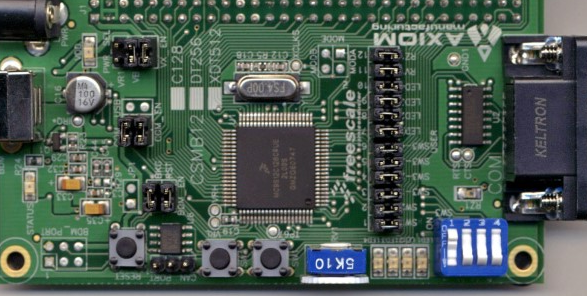
\includegraphics[scale=0.5]{system_setup.png}

        \textbf{System Setup} \\
        NOTE: No hardware other than standard MC9S12C128 module. \\
        Image credit: axman.com/content/csmb-12c128-low-cost-demo-board-freescale-mc9s12c128
    \end{center}

    \begin{center}
        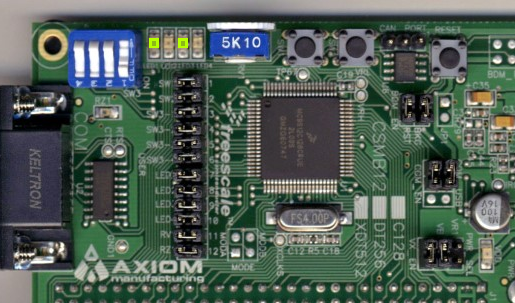
\includegraphics[scale=0.5]{action_shot.png}

        \textbf{Action Shot} \\
        NOTE: No hardware other than standard MC9S12C128 module. \\
        Image credit: axman.com/content/csmb-12c128-low-cost-demo-board-freescale-mc9s12c128
    \end{center}

%-------------------------------------------------------

\sectPart{Public Project Photos}

    \begin{center}
        Our project logo:

        
\includegraphics[scale=0.5]{../../logo.png}

        Our names may be associated with this image.        
    \end{center}    
        
%=======================================================

\end{document}
